% !TEX encoding = UTF-8 Unicode
\documentclass[12pt]{article}

\usepackage[icelandic]{babel}
\usepackage[utf8]{inputenc} 
\usepackage[T1]{fontenc} 
\usepackage{latexsym,amssymb,amsmath}
\usepackage{enumitem}
\usepackage{verbatim}
\usepackage{graphicx}
\usepackage{fancyhdr}
\usepackage{listings}
\usepackage{lstlang05}
\usepackage{color}

\definecolor{lightgray}{rgb}{.9,.9,.9}
\definecolor{darkgray}{rgb}{.4,.4,.4}
\definecolor{purple}{rgb}{0.65, 0.12, 0.82}

\lstdefinelanguage{JavaScript}{
    keywords={typeof, new, true, false, catch, function, return, null, catch, switch, var, if, in, while, do, else, case, break},
    keywordstyle=\color{blue}\bfseries,
    ndkeywords={class, export, boolean, throw, implements, import, this},
    ndkeywordstyle=\color{darkgray}\bfseries,
    identifierstyle=\color{black},
    sensitive=false,
    comment=[l]{//},
    morecomment=[s]{/*}{*/},
    commentstyle=\color{purple}\ttfamily,
    stringstyle=\color{red}\ttfamily,
    morestring=[b]',
    morestring=[b]"
}

\lstset{
    language=JavaScript,
    backgroundcolor=\color{lightgray},
    extendedchars=true,
    basicstyle=\footnotesize\ttfamily,
    showstringspaces=false,
    showspaces=false,
    numbers=left,
    numberstyle=\footnotesize,
    numbersep=9pt,
    tabsize=2,
    breaklines=true,
    showtabs=false,
    captionpos=b
}



\voffset=-1.0in
\hoffset=-0.5in
\textwidth=6in
\textheight=9.0in

\lstset{ %
    language=ampl,                     % the language of the code
    basicstyle=\footnotesize\ttfamily,       % the size of the fonts that are used for the code
    backgroundcolor=\color{white},  % choose the background color. You must add \usepackage{color}
    showspaces=false,               % show spaces adding particular underscores
    showstringspaces=false,         % underline spaces within strings
    showtabs=false,                 % show tabs within strings adding particular underscores
    frame=single,                   % adds a frame around the code
    rulecolor=\color{black},        % if not set, the frame-color may be changed on line-breaks within not-black text (e.g. commens (green here))
    tabsize=2,                      % sets default tabsize to 2 spaces
breaklines=true,                % sets automatic line breaking
    breakatwhitespace=false,        % sets if automatic breaks should only happen at whitespace
    keywordstyle=\color{blue},      % keyword style
    commentstyle=\color{black},   % comment style
    stringstyle=\color{red},      % string literal style
    escapeinside={\%*}{*)},         % if you want to add a comment within your code
    morekeywords={*,...}            % if you want to add more keywords to the set
} 







\begin{document}
\pagestyle{fancy}

\newcommand{\br}{\par}
\newcommand{\substackpar}{}
\newcommand{\substackbr}{,\,}
%\usepackage{makeidx}
\newcommand{\bolddot}{{\mathbf \cdot}}
\newcommand{\C}{{\mathbb  C}}
\newcommand{\Cn}{{\mathbb  C\sp n}}
\newcommand{\crn}{{{\mathbb  C\mathbb  R^n}}}
\newcommand{\R}{{\mathbb  R}}
\newcommand{\Rn}{{\mathbb  R\sp n}}
\newcommand{\Rnn}{{\mathbb  R\sp{n\times n}}}
\newcommand{\Z}{{\mathbb  Z}}
\newcommand{\N}{{\mathbb  N}}
\renewcommand{\P}{{\mathbb  P}}
\newcommand{\Q}{{\mathbb  Q}}
\newcommand{\U}{{\mathbb  U}}
\newcommand{\D}{{\mathbb  D}}
\newcommand{\T}{{\mathbb  T}}
\newcommand{\A}{{\cal A}}
\newcommand{\E}{{\cal E}}
\newcommand{\F}{{\cal F}}
\renewcommand{\H}{{\cal H}}
\renewcommand{\L}{{\cal L}}
\newcommand{\M}{{\cal M}}
\renewcommand{\O}{{\cal O}}
\renewcommand{\S}{{\cal S}}
\newcommand{\dash}{{\sp{\prime}}}
\newcommand{\ddash}{{\sp{\prime\prime}}}
\newcommand{\tdash}{{\sp{\prime\prime\prime}}}
\newcommand{\set }[1]{{\{#1\}}}
\newcommand{\scalar}[2]{{\langle#1,#2\rangle}}
\newcommand{\arccot}{{\operatorname{arccot}}}
\newcommand{\arccoth}{{\operatorname{arccoth}}}
\newcommand{\arccosh}{{\operatorname{arccosh}}}
\newcommand{\arcsinh}{{\operatorname{arcsinh}}}
\newcommand{\arctanh}{{\operatorname{arctanh}}}
\newcommand{\Log}{{\operatorname{Log}}}
\newcommand{\Arg}{{\operatorname{Arg}}}
\newcommand{\grad}{{\operatorname{grad}}}
\newcommand{\graf}{{\operatorname{graf}}}
\renewcommand{\div}{{\operatorname{div}}}
\newcommand{\rot}{{\operatorname{rot}}}
\newcommand{\curl}{{\operatorname{curl}}}
\renewcommand{\Im}{{\operatorname{Im\, }}}
\renewcommand{\Re}{{\operatorname{Re\, }}}
\newcommand{\Res}{{\operatorname{Res}}}
\newcommand{\vp}{{\operatorname{vp}}}
\newcommand{\mynd}[1]{{{\operatorname{mynd}(#1)}}}
\newcommand{\dbar}{{{\overline\partial}}}
\newcommand{\inv}{{\operatorname{inv}}}
\newcommand{\sign}{{\operatorname{sign}}}
\newcommand{\trace}{{\operatorname{trace}}}
\newcommand{\conv}{{\operatorname{conv}}}
\newcommand{\Span}{{\operatorname{Sp}}}
\newcommand{\stig}{{\operatorname{stig}}}
\newcommand{\Exp}{{\operatorname{Exp}}}
\newcommand{\diag}{{\operatorname{diag}}}
\newcommand{\adj}{{\operatorname{adj}}}
\newcommand{\erf}{{\operatorname{erf}}}
\newcommand{\erfc}{{\operatorname{erfc}}}
\renewcommand{\ast}{{\operatorname{\text{?st}}}}
\newcommand{\Lloc}{{L_{\text{loc}}\sp 1}}
\newcommand{\boldcdot}{{\mathbb \cdot}}
%\newcommand{\Cinf0}[1]{{C_0\sp{\infty}(#1)}}
\newcommand{\supp}{{\text{supp}\, }}
\newcommand{\chsupp}{{\text{ch supp}\, }}
\newcommand{\singsupp}{{\text{sing supp}\, }}
\newcommand{\SL}[1]{{\dfrac {1}{\varrho} \bigg(-\dfrac d{dx}\bigg(p\dfrac {d#1}{dx}\bigg)+q#1\bigg)}}
\newcommand{\SLL}[1]{-\dfrac d{dx}\bigg(p\dfrac {d#1}{dx}\bigg)+q#1}
\newcommand{\Laplace}[1]{\dfrac{\partial^2 #1}{\partial x^2}+\dfrac{\partial^2 #1}{\partial y^2}}
\newcommand{\polh}[1]{{\widehat #1_{\C^n}}}
\newcommand{\tilv}{{}}

\newcommand{\sz}{\overline{z}}
\newcommand{\saf}{\overline{f}}
\newcommand{\sw}{\overline{w}}

\newcommand{\pz}{\partial_z}
\newcommand{\psz}{\partial_{\overline{z}}}
%%%

\newcommand{\Nv}{\mbox{${\bf N}$}}

\newcommand{\Bv}{\mbox{${\bf B}$}}


\newcommand{\Tv}{\mbox{${\bf T}$}}


%%%

	\begin{titlepage}
        
        \newcommand{\HRule}{\rule{\linewidth}{0.5mm}} % Defines a new command for the horizontal lines, change thickness here
        
        \center % Center everything on the page
        
        %----------------------------------------------------------------------------------------
        %	HEADING SECTIONS
        %----------------------------------------------------------------------------------------
        
        \textsc{\LARGE Háskóli Íslands}\\[1.5cm] % Name of your university/college
        \textsc{\Large Aðgerðargreining}\\[0.5cm] % Major heading such as course name
        \textsc{\large IÐN401G}\\[0.5cm] % Minor heading such as course title
        
        %----------------------------------------------------------------------------------------
        %	TITLE SECTION
        %----------------------------------------------------------------------------------------
        
        \HRule \\[0.4cm]
        { \huge \bfseries Lokaverkefni - Próftöflubestun}\\[0.4cm] % Title of your document
        \HRule \\[1.5cm]
        
        %----------------------------------------------------------------------------------------
        %	AUTHOR SECTION
        %----------------------------------------------------------------------------------------
        
        \begin{minipage}{0.4\textwidth}
            \begin{flushleft} \large
                \emph{Höfundar:}\\
                Egill Ian Guðmundsson\\
                Hildur Sigurjónsdóttir\\
                Stefán Carl Peiser\\ % Your name
				Unnur Sigurjóns
            \end{flushleft}
        \end{minipage}
        ~
        \begin{minipage}{0.4\textwidth}
            \begin{flushright} \large
                \emph{Umsjónarkennari:} \\
                Tómas Philip Rúnarsson\\
            \end{flushright}
        \end{minipage}\\[4cm]
        
        % If you don't want a supervisor, uncomment the two lines below and remove the section above
        %\Large \emph{Author:}\\
        %John \textsc{Smith}\\[3cm] % Your name
        
        %----------------------------------------------------------------------------------------
        %	DATE SECTION
        %----------------------------------------------------------------------------------------
        
        {\large \today}\\[3cm] % Date, change the \today to a set date if you want to be precise
        
        %----------------------------------------------------------------------------------------
        %	LOGO SECTION
        %----------------------------------------------------------------------------------------
        
       
\includegraphics[scale = 0.3]{hi_logo}\\[1cm] % Include a department/university logo - this will require the graphicx package
        
        %----------------------------------------------------------------------------------------
        
        \vfill % Fill the rest of the page with whitespace
        
    \end{titlepage}

\newpage
\tableofcontents
\newpage
\section{Ágrip}
Bestun próftöflu hefur verið vandmeðfarið verkefni víða um heim síðastliðna áratugi. Verkefnið snýst um að skipuleggja fjöldan allan af prófum yfir takmarkað tímabil. Þessu tímabili er skipt upp í ákveðið marga prófstokka, oftast tvo stokka á dag og þarf verkefnið auk þess að uppfylla fyrirfram ákveðin skilyrði sem kallast skorður.
Skorðurnar eru mismunandi eftir skólum. Þær skorður sem nauðsynlegt er að uppfylla í öllum tilfellum kallast harðar skorður. Sem dæmi um harðar skorður má nefna að sami nemandi getur ekki þreytt tvö próf á sama tíma (í sama prófstokki) og að takmarkaður fjöldi nemenda getur þreytt próf á sama tíma, enda takmarkaður sætafjöldi í boði fyrir hvern stokk. Ef allar harðar skorður eru uppfylltar við bestun próftöflu er litið svo á að lausnin sé lögleg.

\medskip
Aðrar skorður sem hægt er að setja, en teljast ekki nauðsynlegar til þess að leysa verkefnið, eru kallaðar lausar skorður. Dæmi um lausar skorður eru t.d. ákjósanlegur hvíldartími nemenda á milli prófa eða að fjölmenn námskeið séu með próf framarlega á próftímabili. Gefa má þessum lausu skorðum meira eða minna vægi og þar með stilla líkanið til þess að gefa sérsniðnar lausnir. Hægt er að hafa sem mestan hvíldartíma milli prófa , sem fæsta prófstokka , fjölmenn eða erfið námskeið sem fyrst eða taka tillit til allra skorða eins og gert er í lokin.

\medskip
Eins og sést frekar í eftirfarandi köflum er hægt að breyta röðuninni á prófunum með ýmsu móti til að fá niðurstöður frábrugðnar röðun Háskóla Íslands. Hægt er að fækka prófstokkum niður í 13, auka meðalhvíldartíma nemenda um hálfan dag eða færa fjölmennari námskeið framar í töflu. Allt þetta má skoða nánar í niðurstöðum skýrslunnar sem sýnir mismunandi útfærslur á röðun próftöflunnar fyrir vormisseri 2016.
\newpage
\section{Inngangur/bakgrunnur}
Verkefnið sem leyst var af hendi snerist um að hanna líkan sem bestar próftöflu nemenda við Verkfræði- og náttúruvísindasvið Háskóla Íslands. Hugsanlega má rekja þörf verkefnisins til þess að í dag er einn aðili innan háskólans sem sinnir því verkefni að útbúa próftöflur fyrir alla nemendur skólans, þ.e. prófstjóri. Auðvelda mætti ferlið með því að útbúa líkan sem uppfyllir kröfurnar í stað þess að raða prófunum handvirkt. Að sögn kennara ætti líkanið okkar að virka fyrir háskólann í heild sinni, en ekki verður þó farið ítarlegra í það hér.
\medskip
 
Upp voru gefnar þrjár harðar skorður:
\begin{enumerate}
	\item Enginn nemandi getur setið próf samtímis þ.e.a.s. í sama prófstokki.
	\item Próf samkenndra námskeiða skulu vera á sama tíma.
	\item Fjöldi úthlutaðra sæta getur ekki verið meiri en þau sem eru til staðar, í þessu tilfelli 450 sæti.
\end{enumerate}


Auk þess gætu nemendur kosið að hafa smá hvíld á milli prófa og erfiðari próf fyrr á tímabilinu til að einbeita sér frekar að þeim. Einnig verður skoðað hvort hægt sé að koma í veg fyrir að einhverjir hópar innan deildarinnar taki mörg próf á stuttum tíma og þá hvernig væri hægt að leysa það. Óskir kennara varðandi lausnina var að fjölmenn námskeið fengju að hafa prófin snemma á próftímabilinu en stjórnendur skólans vildu sjá lausn sem gæti lágmarkað kostnað vegna húsnæðis auk yfirsetu- og aðstoðarfólks yfir prófatímabilið sem þýðir stytting próftímabilsins eins og hægt er.

\medskip

Í þessu tiltekna líkani er notast við gögn um fallprósentu frá prófstjóra til þess að ákvarða erfiðleika prófs þar sem hærra fall þýðir að öllum líkindum erfiðara próf.

\medskip

Reynt var að hafa sem mesta hvíld milli prófa án þess að lengja próftímabilið um of. Erfiðlega gekk að hafa 
þriggja stokka hvíldartíma eftir öll próf og áætla má að einhverjir nemendur séu í prófum eitthverja daga í röð eða samdægurs.

\medskip


Stilla má líkanið til að lágmarka fjölda stokka, hámarka hvíldartíma, hafa fjölmenn námskeið sem fyrst eða taka mið af þessu öllu. Hvíldartíminn er hafður sem nokkrar skorður sem taka mið af því hversu margir þurfa að vera í árekstri á prófum til þess að líkanið hliðri prófum og auka hvíldartíma. Hvernig skal stilla þessar skorður er fjallað um nánar í seinni köflum. Leggja má enn meiri áherslu á hvíldartíma með því að sleppa markfalli en hægt er að leggja áherslu á lágmörkun prófstokka eða að færa fjölmenn námskeið framar með því að nota tilsett markföll.


\newpage	

\section{Niðurstöður, niðurlag og tillögur}



Líkanið var þróað í nokkrum skrefum. Í öllum tilfellum, nema þess sé sérstaklega getið, var gert ráð fyrir því að nemandi gæti ekki setið tvö próf á sama tíma og að próf samkenndra áfanga séu á sama tíma. Einnig er gert ráð fyrir því að hámarks úthlutunarsæti fyrir hvern prófstokk séu 450 sæti.
Byrjað var á því að kanna hver lágmarksfjöldi prófstokka er sem þarf til að búa til próftöflu með öllum hörðum skorðum sem settar voru hér að undan [graf 1] og einnig hve margir prófstokkarnir yrðu ef fjöldi sæta væri ótakmarkaður [graf 2]. 


\begin{figure}[h]
\centering
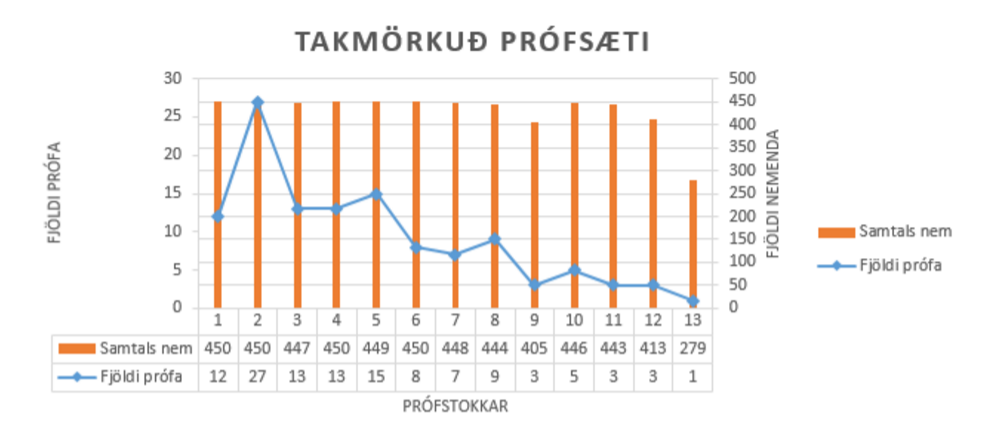
\includegraphics[width = 152mm]{./myndir/graf1}
\caption{Grafið sýnir fjölda nemenda og prófa í hverjum prófstokki. Fjöldi tiltækra sæta í hvern prófstokk var takmarkaður við 450.}
\end{figure}

\begin{figure}[h]
    \centering
    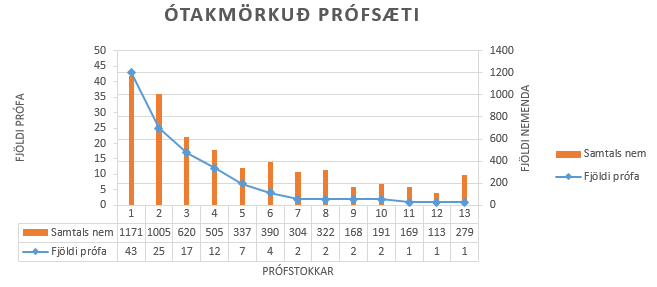
\includegraphics[width = 152mm]{./myndir/graf2}
    \caption{Grafið sýnir fjölda nemenda og prófa í hverjum prófstokki. Fjöldi tiltækra sæta í hverjum prófstokki var ótakmarkaður.}
\end{figure}





Í báðum tilvikum reyndist besta lausnin nota 13 prófstokka, þ.e. engu skipti hvort sætin sem voru tiltæk voru 450 eða að fjöldi sæta væri ótakmarkaður og því styttist próftímabilið ekkert þrátt fyrir að sætaskorðan væri fjarlægð. Hámarksfjöldi sæta sem þyrfti í seinna tilvikinu væri þó 1171 sæti. Dreifing nemenda er jafnari ef fjöldi prófsæta er takmarkaður heldur en þegar fjöldi prófsæta er ótakmarkaður. 
Því næst var fundinn heppilegur mælikvarði á hvíld milli prófa fyrir hópanna 61. Það var gert með því að finna meðalhvíldartíma milli prófa fyrir alla hópa. Fyrir auglýsta próftöflu háskólans fyrir vorið 2016 fengust neðangreind gögn  [graf 3][tafla 1].


\begin{figure}[h]
    \centering
    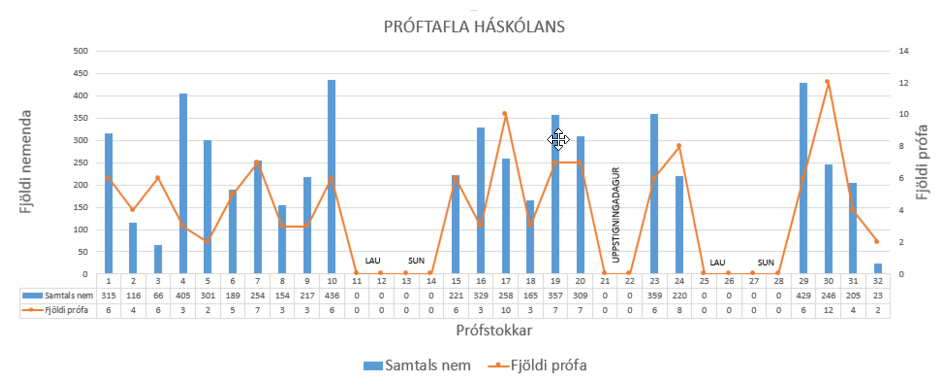
\includegraphics[width = 175mm]{./myndir/graf3}
    \caption{Grafið sýnir fjölda nemenda og prófa í hverjum prófstokki fyrir auglýsta próftöflu Verkfræði- og náttúruvísindasviðs Háskóla Íslands fyrir vormisseri 2016.}
\end{figure}

\begin{table}[h]
    \centering
    \begin{tabular}{l|c|c|}
        \cline{2-3}
        & \multicolumn{1}{l|}{\textbf{Allt prófatímabili}} & \multicolumn{1}{l|}{\textbf{Prófatímabil hópa}} \\ \hline
        \multicolumn{1}{|l|}{\textbf{Fjöldi stokka}} & 6,63                                             & 8,48                                            \\ \hline
        \multicolumn{1}{|l|}{\textbf{Fjöldi daga}}   & 2,90                                             & 3,72                                            \\ \hline
    \end{tabular}
    \caption{Taflan sýnir meðalhvíldartíma hópa miðað við auglýsta próftöflu háskólans}
\end{table}

Fundin var betri lausn með því að byrja á að tryggja að sem fæstir nemendur væru í tveimur prófum sama dag og því næst var lögð áhersla á að sem fæstir nemendur væru í prófum tvo daga í röð. Þegar það líkan var keyrt fengust niðurstöður sem sýndar eru á grafi 4.


\begin{figure}[h]
    \centering
    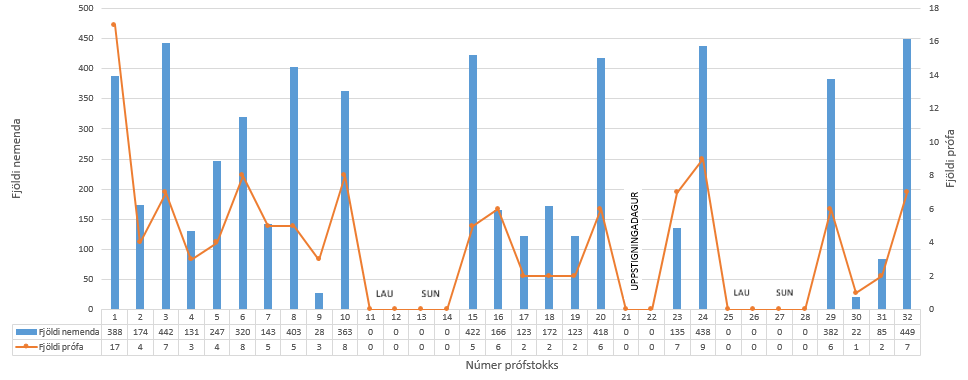
\includegraphics[width = 185mm]{./myndir/graf4}
    \caption{Grafið sýnir fjölda nemenda og prófa í hverjum prófstokki þegar leitað var að lausn betri en auglýst próftafla frá háskólanum gaf.}
\end{figure}

\newpage

Þessi lausn gefur að meðalhvíldartími frá byrjun próftímabils til síðasta prófs er lengri og jafnframt er meðalhvíldartími nemenda frá fyrsta og síðasta prófi fyrir hvern hóp lengri [tafla 2]. 
Fjöldi nemenda er rokkandi, allt frá 22 nemendum og upp í 449 nemendur. Þessi lausn væri hentug nemendum sem kjósa góðan hvíldartíma á milli prófa en væri síður kostur fyrir stjórnendur skólans.


\begin{table}[h]
    \centering
    \begin{tabular}{l|c|c|}
        \cline{2-3}
        & \multicolumn{1}{l|}{\textbf{Allt prófatímabili}} & \multicolumn{1}{l|}{\textbf{Prófatímabil hópa}} \\ \hline
        \multicolumn{1}{|l|}{\textbf{Fjöldi stokka}} & 7,82                                             & 9,25                                            \\ \hline
        \multicolumn{1}{|l|}{\textbf{Fjöldi daga}}   & 3,48                                             & 4,08                                            \\ \hline
    \end{tabular}
    \caption{Taflan sýnir meðalhvíldartíma hópa við bættan hvíldartíma milli prófa.}
\end{table}


Til þess að lágmarka fjölda prófstokka var líkanið hannað þannig að prófunum var raðað í fremstu prófstokkana og þar með tryggði það einnig að nemendur klára prófin á sem styðstum tíma. 

\newpage

\begin{figure}[h]
    \centering
    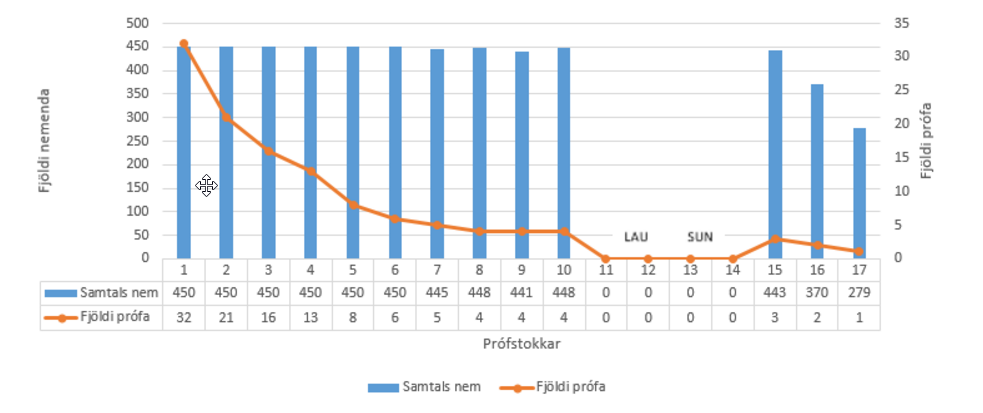
\includegraphics[width = 175mm]{./myndir/graf5}
    \caption{Grafið sýnir fjölda nemenda og prófa í hverjum prófstokki þegar fengin var lausn við lágmörkun prófstokka.}
\end{figure}

Á grafinu [5] sést að fyrstu sex prófstokkarnir hafa flesta nemendur eða 450 talsins og eru því fullnýttir. Einungis í prófum sem þreytt eru í síðustu tveimur stokkunum er fjöldi nemenda færri en 400 en í stokki 16 eru 370 nemendur og í síðasta stokknum er fjöldi nemenda 279.
Hvíldartíminn á milli prófa styttist en meðalhvíldartími frá byrjun próftímabils til síðasta prófs er 0,87 dagar og meðalhvíldartími frá fyrsta prófi til síðasta prófs fyrir hvern hóp er 0,94 dagar. Þar með sést að meðalhvíldartíminn frá byrjun til enda próftímabils styttist um 2,61 daga og meðalhvíldartími frá fyrsta prófi til síðasta prófs styttist um 3,14 daga. 


\begin{table}[h]
    \centering
    \begin{tabular}{l|c|c|}
        \cline{2-3}
        & \multicolumn{1}{l|}{\textbf{Allt prófatímabili}} & \multicolumn{1}{l|}{\textbf{Prófatímabil hópa}} \\ \hline
        \multicolumn{1}{|l|}{\textbf{Fjöldi stokka}} & 2,25                                             & 2,47                                            \\ \hline
        \multicolumn{1}{|l|}{\textbf{Fjöldi daga}}   & 0,87                                             & 0,94                                            \\ \hline
    \end{tabular}
    \caption{Taflan sýnir meðalhvíldartíma hópa þegar fjöldi  prófstokka var lágmarkaður.}
\end{table}

Kennarar vildu sjá próf fjölmennari námskeiða fyrr á tímabilinu og var líkaninu breytt til þess að koma á móts við óskir þeirra. Graf sex sýnir breytingu á dreifingu nemenda í prófstokka.


\begin{figure}[h]
    \centering
    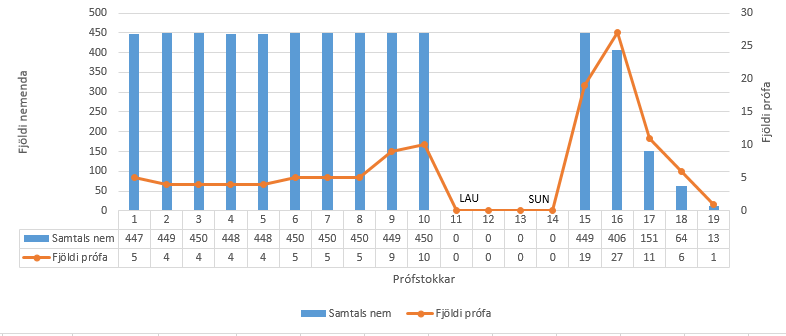
\includegraphics[width = 140mm]{./myndir/graf6}
    \caption{Grafið sýnir fjölda nemenda og prófa í hverjum prófstokki. Hér er fjölmennustu námskeiðunum raðað fremst í prófstokkana.}
\end{figure}

\newpage

Við það að raða prófum fjölmennustu námskeiða fremst á tímabilið eykst meðalhvíldartími hópa miðað við þá niðurstöðu er fékkst þegar fjölda prófstokka var lágmarkaður [tafla 3] en er þó töluvert minni en meðalhvíldartími auglýstrar próftöflu fyrir deildina vorið 2016 [tafla 1]. Niðurstöður meðalhvíldartíma hópa við þessa lausn má sjá í töflu 4.
Dreifing nemenda yfir tímabilið er ekki ósvipuð og þegar fjöldi prófstokka var lágmarkaður, en heildarfjöldi nýttra prófstokka, þegar prófum fjölmennustu námskeiðunum er raðað fremst í próftöfluna, er 19. Síðustu þrír prófstokkarnir telja færri en 150 nemendur en aðrir nýttir prófstokkar fleiri en 400 nemendur.


\begin{table}[h]
    \centering
    \begin{tabular}{l|c|c|}
        \cline{2-3}
        & \multicolumn{1}{l|}{\textbf{Allt prófatímabili}} & \multicolumn{1}{l|}{\textbf{Prófatímabil hópa}} \\ \hline
        \multicolumn{1}{|l|}{\textbf{Fjöldi stokka}} & 3,27                                             & 3,35                                            \\ \hline
        \multicolumn{1}{|l|}{\textbf{Fjöldi daga}}   & 1,41                                             & 1,42                                            \\ \hline
    \end{tabular}
    \caption{Taflan sýnir meðalhvíldartíma hópa þegar fjölmennustu námskeiðunum er raðað fremst í prófstokka.}
\end{table}

Að lokum var stillt upp líkani sem talið er gefa bestu lausn fyrir nemendur, kennara og stjórnendur skólans.  Við líkangerðina var í fyrsta lagi haft í huga að fjölmenn námskeið væru eins framarlega á próftímabili og unnt væri. Í öðru lagi var reynt eftir fremsta megni að tryggja að nemendur væru ekki í tveimur prófum sama dag og að þeir hefðu að minnsta kosti einn prófstokk í hvíld á milli prófa helst þó heilan dag. Í þriðja lagi voru próf með háa fallprósentu sett eins framarlega á próftímabil og unnt var. Að lokum var einnig haft í huga að stjórnendur skólans vilja spara kostnað og þar með var reynt að minnka fjölda nýttra stokka. 


\begin{figure}[h]
    \centering
    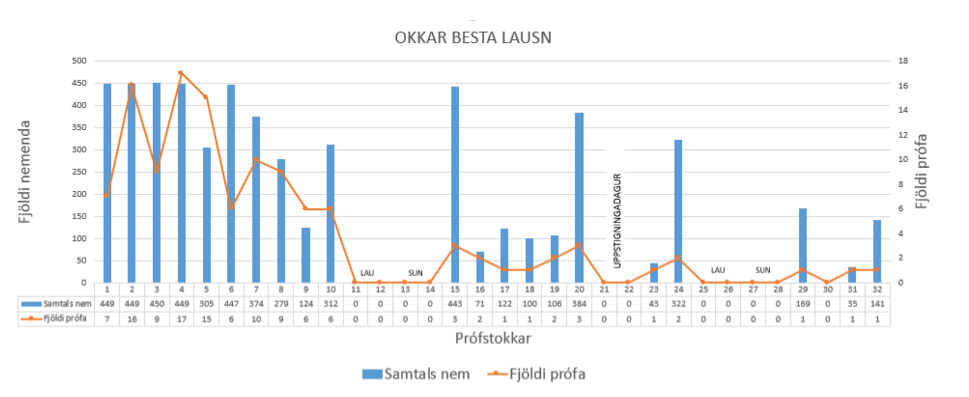
\includegraphics[width = 150mm]{./myndir/graf7}
    \caption{Grafið sýnir hagkvæmnustu lausn sem fengin var samkvæmt þeim skorðum sem settar voru.}
\end{figure}

\newpage
\begin{table}[h]
    \centering
    \begin{tabular}{l|c|c|}
        \cline{2-3}
        & \multicolumn{1}{l|}{\textbf{Allt prófatímabili}} & \multicolumn{1}{l|}{\textbf{Prófatímabil hópa}} \\ \hline
        \multicolumn{1}{|l|}{\textbf{Fjöldi stokka}} & 5,98                                             & 7,13                                            \\ \hline
        \multicolumn{1}{|l|}{\textbf{Fjöldi daga}}   & 2,56                                             & 3,05                                            \\ \hline
    \end{tabular}
    \caption{Taflan sýnir meðalhvíldartíma hópa miðað við hagkvæmustu lausn. }
\end{table}

Líkanið er betra en lausn Háskóla Íslands að því leyti að það notar einum færri prófstokk og þar með minnkar kostnaður við prófhald, sem um nemur yfirsetufólki og kennslustofum. Hvíldartími er ögn minni, u.þ.b. hálfur dagur, heldur en auglýsta lausnin en er þó ásættanlegur fyrir nemendur. 

\medskip
Líkanið var hannað þannig að ef fjöldi nemenda sem taka próf í tveimur mismunandi fögum var nægur átti lausnin að hafa ákveðinn fjölda stokka á milli. Eftir nokkrar prófanir kom í ljós að hentugast var, til þess að tryggja sem mestan heildarhvíldartíma, að hafa a.m.k. einn stokk á milli prófa ef fjöldi nemenda í báðum fögum var meiri en eða jafn tveimur,  tvo stokka ef fjöldi nemenda var meiri en eða jafn níu og þrjá stokka hið minnsta ef fjöldi nemenda var meiri en eða jafn 15. Þar með tókst að tryggja að sem flestir nemendur fái að minnsta kosti þriggja stokka frí, þ.e.a.s. einn og hálfan dag, á milli prófa. 

\medskip
Þar að auki voru “fjölmenn” námskeið færð framar á próftímabilið en það var gert að ósk kennara því það hentar þeim betur til yfirferðar. Hægt var að hafa allra stærstu námskeiðin fremst í uppröðuninni en það reyndist óhagstætt þar sem önnur fjölmenn námskeið lentu í mun verri stöðu. Því var ákveðið að nota lausn sem tekur tillit til heildarinnar en ekki einungis stærstu námskeiðanna.

\medskip
Einnig hefur verið tryggt að próf með hærri fallprósentu, þ.e.a.s. strembin próf, eru framarlega í uppröðuninni sem nemendum hefur þótt ákjósanlegt. 
Að endingu var líkanið fyrir bestu lausn keyrt fyrir mismunandi fjölda prófstokka. Ekki fékkst lögleg lausn þegar prófstokkum var fækkað. Hinsvegar, þegar þeim var fjölgað fengust mismunandi lausnir sem gáfu eftirfarandi hvíldartíma.

\newpage

Að lokum var prófað hvernig hvíldartíminn breyttist þegar prófstokkum var fjölgað eða fækkað. Í ljós kom að 32 prófstokkar var algjört lágmark en aftur á móti var hægt að bæta við prófstokkum. Þegar bætt var við prófstokkum fannst að hámarksfjöldi stokka sem gæfi nýja lausn í próftöflubestuninni væri 38 stokkar. 

\begin{figure}[h]
    \centering
    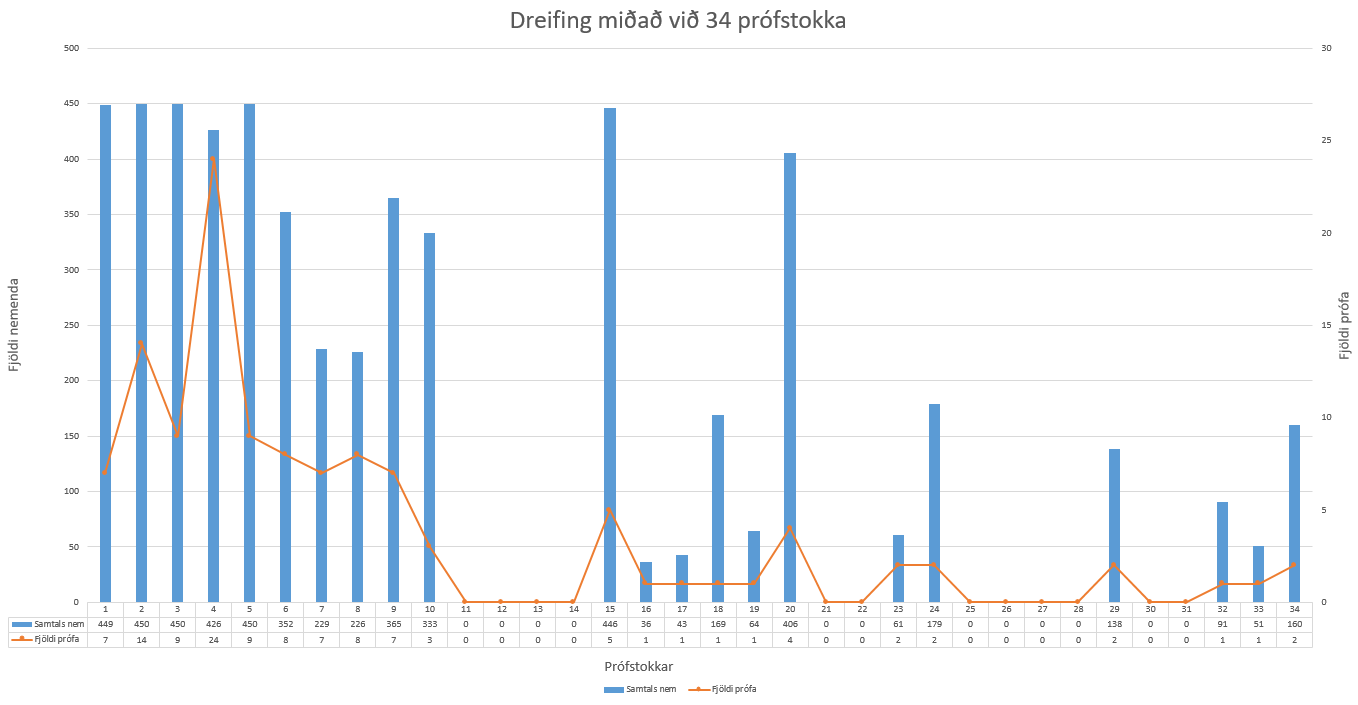
\includegraphics[width = 180mm]{./myndir/graf8}
    \caption{Grafið sýnir hagkvæmnustu lausn fyrir 34 prófstokka.}
\end{figure}

\begin{table}[h]
    \centering
    \begin{tabular}{l|c|c|}
        \cline{2-3}
        & \multicolumn{1}{l|}{\textbf{Allt prófatímabili}} & \multicolumn{1}{l|}{\textbf{Prófatímabil hópa}} \\ \hline
        \multicolumn{1}{|l|}{\textbf{Fjöldi stokka}} & 6,25                                             & 5,08                                            \\ \hline
        \multicolumn{1}{|l|}{\textbf{Fjöldi daga}}   & 2,62                                             & 2,13                                            \\ \hline
    \end{tabular}
    \caption{Taflan sýnir meðalhvíldartíma hópa miðað við 34 prófstokka.}
\end{table}



\newpage
\begin{figure}[h]
    \centering
    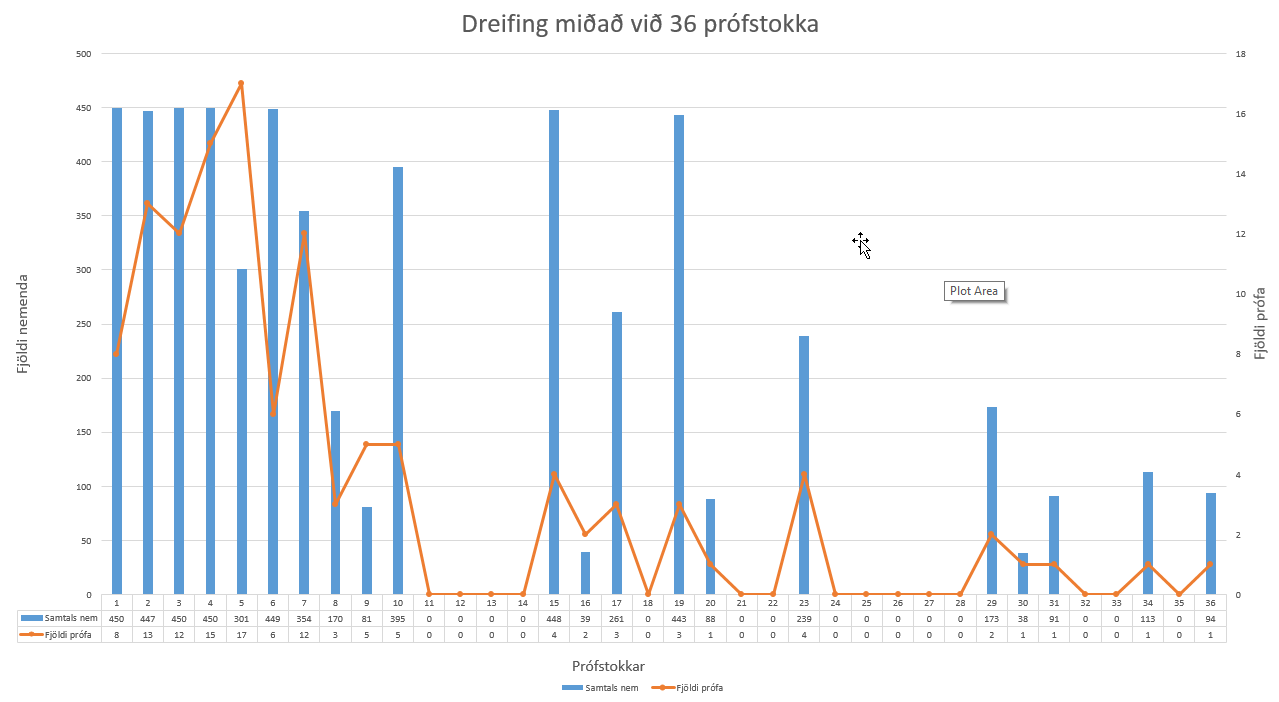
\includegraphics[width = 180mm]{./myndir/graf9}
    \caption{Grafið sýnir hagkvæmnustu lausn fyrir 36 prófstokka.}
\end{figure}

\begin{table}[h]
    \centering
    \begin{tabular}{l|c|c|}
        \cline{2-3}
        & \multicolumn{1}{l|}{\textbf{Allt prófatímabili}} & \multicolumn{1}{l|}{\textbf{Prófatímabil hópa}} \\ \hline
        \multicolumn{1}{|l|}{\textbf{Fjöldi stokka}} & 5,87                                             & 4,85                                            \\ \hline
        \multicolumn{1}{|l|}{\textbf{Fjöldi daga}}   & 2,49                                             & 2,06                                            \\ \hline
    \end{tabular}
    \caption{Taflan sýnir meðalhvíldartíma hópa miðað við 36 prófstokka.}
\end{table}

\newpage

\begin{figure}[h]
    \centering
    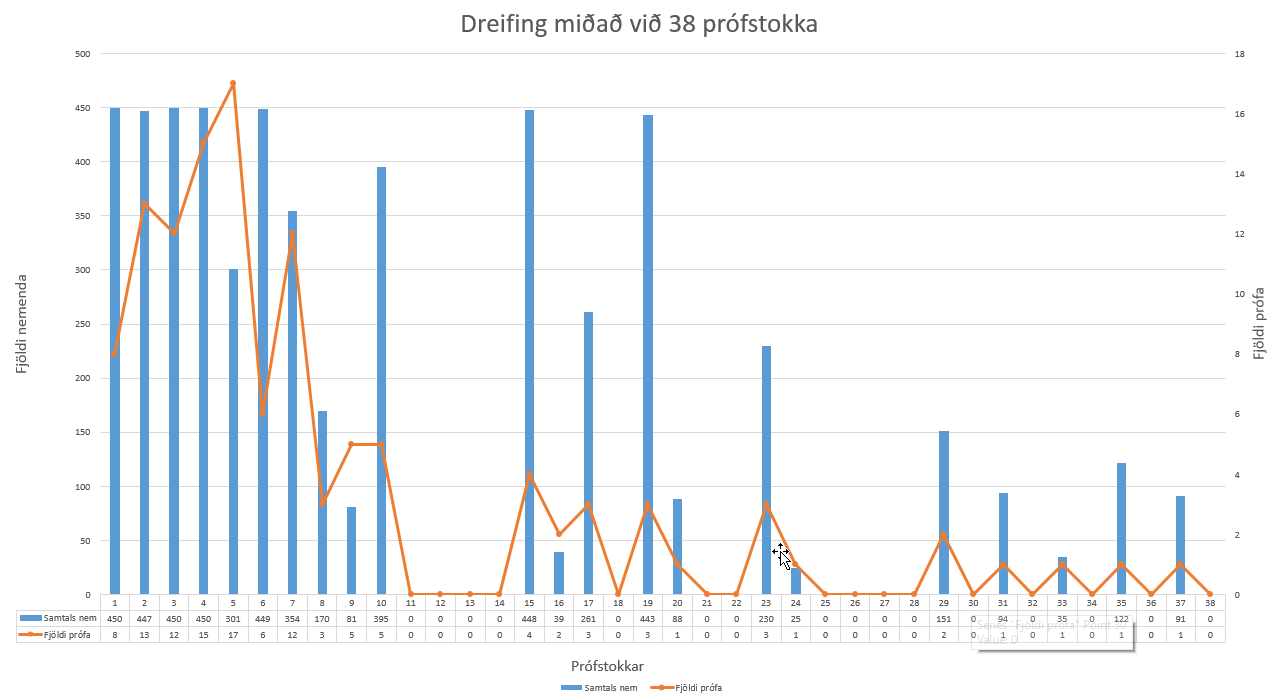
\includegraphics[width = 180mm]{./myndir/graf10}
    \caption{Grafið sýnir hagkvæmnustu lausn fyrir 38 prófstokka.}
\end{figure}

\begin{table}[h]
    \centering
    \begin{tabular}{l|c|c|}
        \cline{2-3}
        & \multicolumn{1}{l|}{\textbf{Allt prófatímabili}} & \multicolumn{1}{l|}{\textbf{Prófatímabil hópa}} \\ \hline
        \multicolumn{1}{|l|}{\textbf{Fjöldi stokka}} & 6,07                                             & 4,96                                            \\ \hline
        \multicolumn{1}{|l|}{\textbf{Fjöldi daga}}   & 2,62                                             & 2,13                                            \\ \hline
    \end{tabular}
    \caption{Taflan sýnir meðalhvíldartíma hópa miðað við 38 prófstokka.}
\end{table}


Hér sést að ef prófstokkunum er fjölgað í annaðhvort 34 eða 38 þá eykst meðalhvíldartími yfir allt prófatímabilið. Aftur á móti bitnar það verulega á ákveðnum hópum þar sem meðalhvíldartími frá fyrsta til síðasta prófs hópa minnkar alls staðar. Hinsvegar, fyrir 36 stokka verður nýtingin það léleg að hvíldartíminn minnkar bæði frá upphafi próftímabils og frá fyrsta prófi hópa. Hafa ber í huga að eftir því sem prófstokkum fjölgar þá jafnframt eykst kostnaður, þar sem nýta þarf stofur yfir lengra tímabil ásamt því að greiða þarf yfirsetufólki og kennarar þurfa að vera til staðar í stað þess að geta nýtt tímann til prófyfirferðar.
\newpage

\section{Aðferðir}

Áður en hægt var að setja líkanið upp í AMPL þurfti að færa skorðurnar og markföll á stærfræðilegt form. Í eftirfarandi uppsetningu er notast við það táknmál að e er mengi staka úr vigrinum \verb|examSlots| og c er mengi staka úr vigrinum \verb|cidExam|. Einnig samanstendur \verb|slot| fylkið af  ákvörðunarbreytunum verkefnisins (köllum það x héðan í frá) og n er stærð hvers vigurs um sig. Notað er k  til að tákna mengi staka úr \verb|cidCount| þar sem hvert stak er fjöldi nemenda í námskeiði k, l táknar mengi staka úr \verb|cidDifficulty| sem inniheldur fallprósentu námskeiðs l, m er mengi staka úr \verb|cidCommon| og s er fjöldi nemenda á Verk- og Náttúrufræðisviði Háskóla Íslands.  Markfallið \verb|earlyExams| má setja fram sem:

$$\min \sum_{j \in c, i \in e} x_{ji} \cdot i^8$$

Þar sem reynt er að lágmarka fjölda námskeiða sem lendir aftarlega í prófröðun. Eftir því sem stokkurinn er aftar (og þá i stærra) verður mun óhagkvæmara að setja prófið þar. Skoðum næst markfallið \verb|bigExamEarly| og uppsetningu þess:

$$\min \sum_{j \in c, i \in e} x_{ji} \cdot \left( k_j \cdot i^2 \right)^4$$

Hérna er nemendafjöldinn margfaldaður við prófstokksnúmer í öðru veldi og það síðan hafið upp í fjórða veldi. Seinasta markfallið, \verb|totalSlots|, er það sem er notað til að finna hagkvæmustu lausn:

$$\min \sum_{j \in c, i \in e} x_{ji} \left( b_j \cdot \dfrac{(d_j + 1)^4}{s} \right) \cdot \left( \sqrt[4]{i} \right)$$

Notast var við brotið til að ákveða hlutfallslegt vægi námskeiðs. Eftir því sem það er fjölmennara og erfiðara er það sett í fremri prófstokka. Síðan er það margfaldað með fjórðu rót af númeri prófstokks til að færa námskeið framar í próftöflu. Valið var fjórða veldi á erfiðleikastiginu til að koma til móts við nemendafjölda. Með þessu helst ákveðið jafnvægi að minni námskeiðin lenda ekki allt of aftarlega. Einnig var fjórða rótin valin til þess að raða prófunum framarlega en ef það var haft hærra var fjölmennustu prófunum raðað í fyrstu stokkana á kostnað allra annarra prófa.

\medskip

Skorðurnar eru fleiri að tölu og sú fyrsta er \verb|examClashes| sem sér til þess að engir nemendur eru í prófi á sama tíma:

$$\sum_{ i \in e \, h,j \in c: m_{hj} > 0} x_{hi} + x_{ji} <= 1$$

\verb|hasExam| skorðan

\begin{figure}[h]
	\centering
	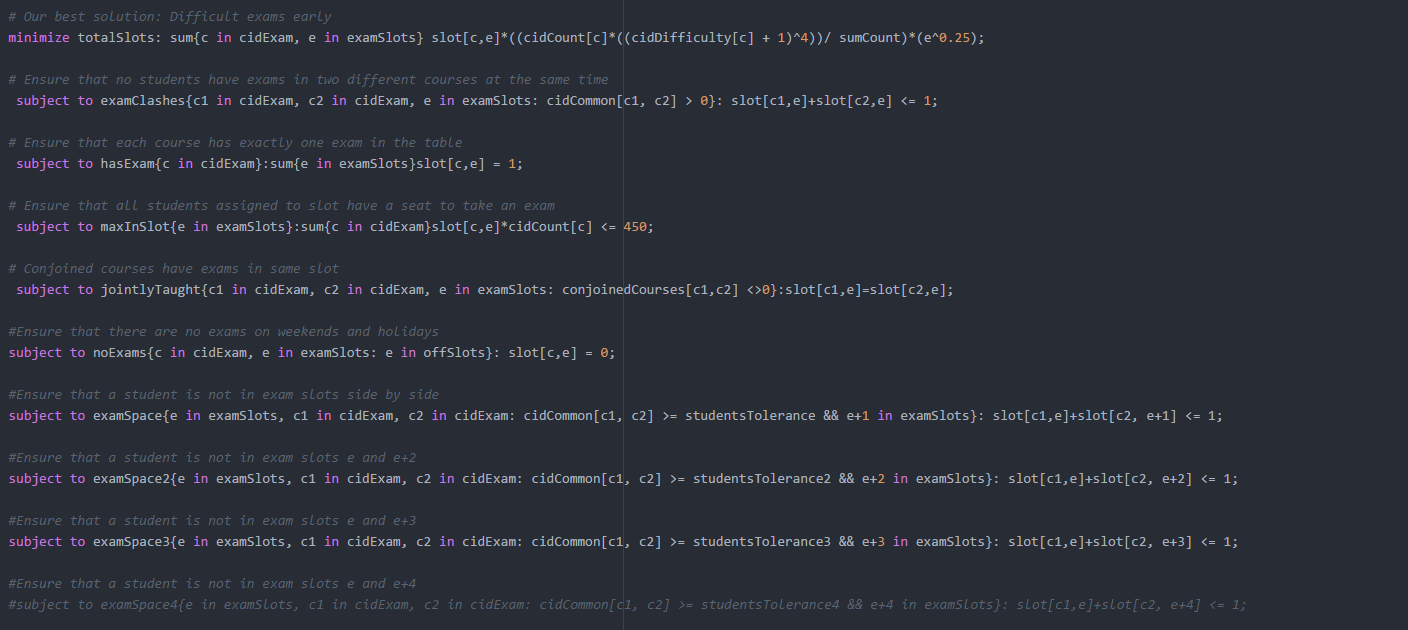
\includegraphics[width = 20cm]{tmp.png}
\end{figure}

\medskip

Notast var við bæði \texttt{AMPL} og \texttt{JavaScript} forritun til að búa til líkan og vinna úr upplýsingum sem úr því fengust. Mælt er með að nota \texttt{GLPK} forritasafnið til að þýða líkanið yfir á \texttt{.lp} skráartegund, \texttt{Gurobi} til að keyra \texttt{.lp} líkanið og fá lausn ásamt því að nota \texttt{Node.js} til að keyra \texttt{JavaScript} forritið sem fylgir.

\medskip

Byrjað var á að safna saman gögnum í gagnaskrá (\texttt{profrodun2016.dat}).  Þar voru skráðir þeir prófstokkar sem ekki eru nýttir til prófa þ.e.a.s. þeir stokkar sem lenda á helgum, á uppstigningardegi eða öðrum frídögum. Þessir prófstokkar voru skilgreindir í menginu \texttt{offSlots} í skránni. Því næst voru gögn fyrir fallprósentu sett inn, sem fengust hjá prófstjóra, en fallprósentan var skilgreind sem  \texttt{cidDifficulty}.  Fallprósentan er nýtt til þess að geta sett próf með hárri fallprósentu, erfið próf, framarlega á tímabilið. Þá var bætt inn fylki \texttt{conjoinedCourses} fyrir samkennd námskeið. Þau námskeið sem eru samkennd hafa einn þar sem lína fyrra námskeiðs sker dálk seinni námskeiðs, annars núll ef þau eru ekki samkennd. Heiti námskeiða er geymt í vigrinum \texttt{cidExam}. Mengin \texttt{group[x]}, þar sem \texttt{x} er á bilinu einn upp í 61, geyma námskeið sem tilheyra kjörsviði \texttt{x}.   Fylkið \texttt{cidCommon} geymir upplýsingar um fjölda þeirra nemenda sem eru í sameiginlegum námskeiðum. 

\medskip

Inni í líkaninu (\texttt{profrodun2016.mod}) má stilla \texttt{n} til að fjölga eða fækka dögum sem eru á próftímabilinu. Einnig þarf að stilla \texttt{sumCount} í samræmi við nemendafjölda. Að lokum er hægt að stilla “studentsTolerance” fyrir það hversu háan fjölda nemenda, sem ekki uppfylla skorðu, þarf svo að skorða sé þó ennþá virk. Hægt er að stilla þrjú “studentsTolerance” svo að þolmörkin geti verið mismunandi fyrir hverja skorðu. 
Til þess að keyra líkanið er byrjað á að velja þær skorður sem eiga að vera inni, þ.e. valið hvað lausnin þarf að uppfylla og einnig er valið það markfall sem við á. Hinar skorðurnar og markföllin eru kommentuð út með \# tákni. 

\medskip

\texttt{JavaScript} reiknirit (\texttt{dataProcessing.js}) var notað til þess að reikna meðalhvíldartíma milli prófa, í stokkum og dögum,  annars vegar frá upphafi prófatímabils og hins vegar frá fyrsta prófi hóps til síðasta prófs. Gögnin sem reikna á úr þarf að setja upp í gagnaskrá (\texttt{dataFile.js}). Undir hverja próftöfluröðun þarf eitt fylki með tveimur línum. Fyrri línan er strengjafylki með heiti námskeiða og seinni línan er heiltöluvigur með viðeigandi prófstokksnúmer fyrir hvert fag. Einnig þarf að setja inn strengjafylki fyrir hvern hóp með viðeigandi námskeiðsheitum. Mælt er með því að nota \texttt{Excel }eða ritil með virkni fyrir reglulegar segðir, eins og \texttt{Atom}, til að vinna úr gögnum úr líkaninu eða mögulega að skrifa nýtt fall til þess. Passa þarf að flytja gögnin yfir í gagnavinnsluskrána með \texttt{export} skipun.

\medskip
Innan í gagnavinnsluskránni (\texttt{dataProcessing.js}) þarf að taka á móti gögnunum með \texttt{require }skipun. Þegar það er komið má notfæra sér \texttt{processDataMatrix()} fallið til að reikna út meðalbiðtíma fyrir alla hópana með gefinni lausn. Frekari lýsing á fallinu og virkni þess má finna í gagnavinnsluskránni.
Reikniritin má finna í viðauka skýrslunnar. Búið er að gefa lýsingar á öllum föllum í gagnavinnsluskránum og sjá má útskýringar á öllum skorðum og ákvörðunum sem hafa verið teknar varðandi hvernig besta eigi próftöfluna.

\newpage

\section{Almenn umfjöllun}

Líkanið er sérhannað til þess að eiga við gerð próftaflna en það má nýta í önnur verkefni sem raða atburðum niður á tíma. Ef haldin er ráðstefna eða syrpa af fundum á stuttum tíma þar sem ákveðnir aðilar verða að vera viðstaddir í ákveðnum fundum eða fyrirlestrum mætti nota þetta líkan til þess að raða fundunum og fyrirlestrunum í dagskrá. Einnig mætti nota líkanið, eða hluta úr því, til að raða stundatöflum fyrir námskeið. Þá væri hægt að endurskrifa skorðurnar til þess að hafa sem minnst bil milli námskeiða í stundatöflu og hafa aðrar skorður til að raða námskeiðum sem minnst á kvöldin.


Eflaust eru til fleiri verkefni þar sem þarf að raða ákveðna tíma á ákveðna atburði (vaktaskipulag og annað slíkt) en líklega þyrfti að breyta skorðum að verulegu leyti eða bæta nýjum skorðum við til að verða við slíkum verkefnum.


\medskip
Þegar verið var að reikna hvíldartíma fyrir hópa í þessu verkefni var eingögnu notast við hvíldartíma fyrir hvern hóp og hver hópur hafði jafnmikið vægi. Til að auka nákvæmni á því hversu mikill hvíldartími ávinnst væri betra að hafa fjölda nemenda í hverjum hópi og taka vegið meðaltal með tilliti til þess. Einnig væri hægt að raða námskeiðum sem fjölmennir hópar taka á “betri” staði í röðuninni með skorðum sem nota fjölda nemenda í hópum. Einnig má nota aðrar leiðir til að meta erfiðleika en fallprósenta. Að öllum líkindum eru til betri aðferðir og mögulega til gögn um erfiðleikastig en ekki var notast við slíkt í þessu líkani.

\section{Heimildir}

Gögn sem nýtt voru við gerð verkefnisins:
\begin{itemize}
	\item Gögn sem fylgdu verkefnalýsingu
	\item Gögn um fallprósentu fengin hjá prófstjóra
	\item AMPL handbók
\end{itemize}

\newpage

\section{Viðauki}

\subsection{AMPL kóði}

\texttt{profrodun2016.mod}
\lstinputlisting[language=ampl]{../profrodun2016Latex.mod}

\subsection{Javascript kóði}

\texttt{dataProcessing.js}
\lstinputlisting[language=Javascript]{../waitTimeProcessing/dataProcessing.js}

\end{document}



%%%